\documentclass[11pt]{article}

\usepackage{a4wide}
\usepackage[utf8]{inputenc}
\usepackage[russian]{babel}
\usepackage{graphicx}
\usepackage{indentfirst} 
\usepackage{amsmath}
\usepackage{amssymb}
\usepackage{amsthm}
\usepackage{floatflt}

\newtheorem{Th}{Теорема}

\newcommand\Real{\mathbb{R}} 
\newcommand\PS{\mathcal{P}}
\newcommand\X{\mathcal{X}} 
\newcommand\Sup[2]{\rho( #1 \, | \, #2 )}
\newcommand\Conv[1]{{\rm conv}\{ #1 \}}
\newcommand\Sgn{{\rm sgn \,}}


\begin{document}

\thispagestyle{empty}

\begin{center}
\ \vspace{-3cm}


\includegraphics[width=0.5\textwidth]{msu.eps}\\
{\scshape Московский государственный университет имени М.~В.~Ломоносова}\\
Факультет вычислительной математики и кибернетики\\
Кафедра системного анализа

\vfill

{\LARGE Отчёт по самому важному предмету}

\vspace{1cm}

{\Huge\bfseries <<Практикум по оптимальному управлению>>}
\end{center}

\vspace{1cm}

\begin{flushright}
  \large
  \textit{Студент 315 группы}\\
  Д.\,М.~Сотников

  \vspace{5mm}

  \textit{Руководитель практикума}\\
  к.ф.-м.н., доцент П.\,А.~Точилин
\end{flushright}

\vfill

\begin{center}
Москва, 2020
\end{center}

\newpage
\part{Теоретическая часть}
\section{Постановка задачи}

Дана система обыкновенных дифференциальных уравнений
\[
\dot{x}\left (t\right ) = A x\left (t\right ) + B u\left (t\right ) + f, \quad t \in [t_0, +\infty),
\]
где $x(t) \in \Real^2, \ u(t) \in \Real^2, \ A \in \Real^{2 \times 2}, \ B \in \Real^{2 \times 2},
 \ f \in \Real^2$, а значения функции управления $u(t) \in \PS \quad \forall t \in [t_0, +\infty)$.

Множество допустимых управлений имеет вид 
$$ \PS = \left\{ x \in \Real^2 \colon \ x_1^2 + a x_2^2 \leq b, \ ax_1^2 + x_2^2 \leq b \right\}, \quad a,b > 0.$$
Будем считать, что $a > 1$, в противном случае сделаем замену $a = \frac{1}{a}, \ b = \frac{b}{a}$.

Начальное множество зачений фазового вектора: $$\X_0 = \mathbb{B}(x_0, r_0).$$

Терминальное множество: $$\X_1 = \Conv{x_1^{\left(1\right)}, \ldots, x_1^{\left(n\right)}} + \mathbb{B}(0, \epsilon), \quad n \in \mathbb{N}.$$

Необходимо численно решить задачу быстродействия, то есть перевести систему из множества $\X_0$ в множество $\X_1$,
минимизируя время перемещения $(t_1 - t_0)$. При этом, поскольку система является линейной и автономной, будем считать, что $t_0 = 0$.


\newpage
\section{Принцип максимума Понтрягина}
Решение задачи опирается на принцип максимума Понтрягина для линейных систем.

\begin{Th}[Принцип максимума Понтрягина] 
Пусть $(x^*(\cdot), \ u^*(\cdot))$ --- оптимальная пара. Тогда существует отличная от нуля функция 
$\psi(\cdot)$, для которой выполнено
\begin{enumerate}
\item $\langle \psi(t), \ Bu^*(t) \rangle = \Sup{\psi(t)}{B \PS}$ для почти всех $t \in [0, t_1^*]$; 
\item $\langle \psi(0), \ x^*(0) \rangle = \Sup{\psi(0)}{\X_0}$;
\item $\langle -\psi(t_1^*), x^*(t_1^*) \rangle = \Sup{-\psi(t_1^*)}{\X_1}$.
\end{enumerate}
При этом функция $\psi(\cdot)$ является решением сопряженной системы $\dot \psi(t) = -A^T\psi(t)$.
\end{Th}

Таким образом задача сводится к поиску функций, удовлетворяющим принципу максимума, и нахождению оптимальной перебором по $t_1$.

Для проверки пунктов теоремы необходимо знать опорные функции множеств $\X_0, \ \X_1, \ \PS$, 
которые можно найти аналитически.

\newpage
\section{Вычисление опорных функций}
В этом разделе приведено аналитическое вычисление опорных функций для начального, терминального множества и множества допустимых управлений.

Поскольку $\X_0$ является шаром, его опорная функция известна и имеет вид
$$\Sup{l}{\X_0} = \Sup{l}{\left\{x_0\right\}} + \Sup{l}{\mathbb{B}(0, r_0)} = 
\langle l, \ x_0 \rangle + r_0\|l\|.$$

Для вычисления опорной функции $X_1$ воспользуемся свойством линейности $\rho$ по второму аргументу и 
тем, что опорная функция для выпуклой комбнации точек является максимумом скалярных произведений
вектора $l$ на эти точки:
$$\Sup{l}{\X_1} = \Sup{l}{\Conv{x_1^{\left(1\right)},, \ldots, x_1^{\left(n\right)}}} + \Sup{l}{\mathbb{B}(0, \epsilon)} =
\max_{i = 1,\ldots,n} \langle l, \ x_1^{\left(i\right)} \rangle + \epsilon \|l\|.$$

Множество $\PS$ является пересечением двух эллипсоидов \\
$$x_1^2 + a x_2^2 \leq b,$$
$$ax_1^2 + x_2^2 \leq b,$$
где $a > 1, \ b > 0$. \\
\noindent
\parbox[b][5cm][t]{50mm}{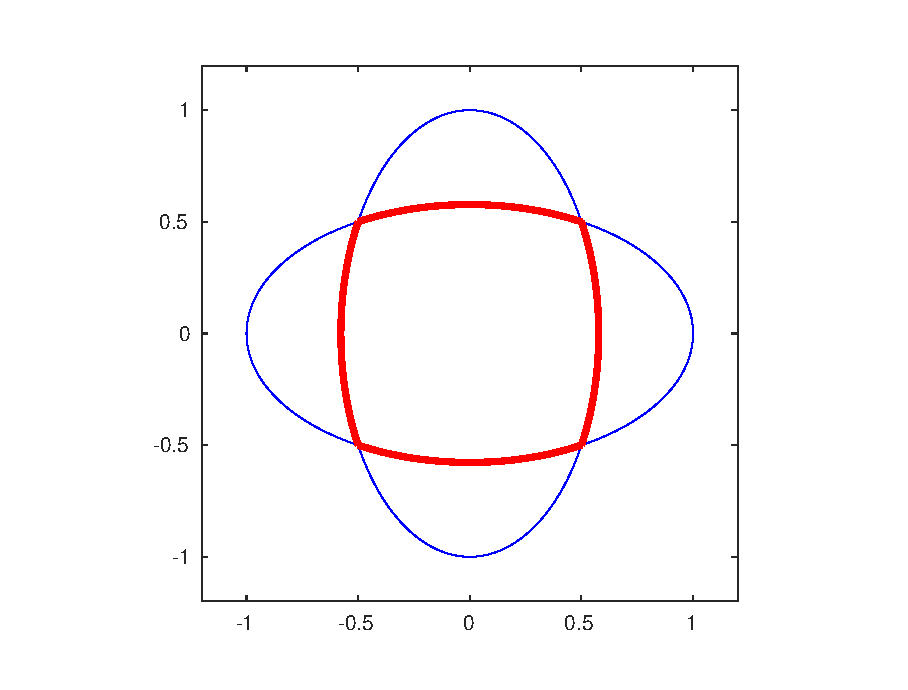
\includegraphics[height=50mm]{P_set.eps}}
\hfill
\parbox[b][5cm][t]{90mm}{
На рисунке множество $\PS$ отмечено красным. Видно, что в силу симметрии достаточно найти опорную
функцию и опорный вектор только в случае, когда $l$ лежит в первом октанте.

Используя функцию Лагранжа, находим условный экстремум на эллипсе $x_1^2 + a x_2^2 = b$:
$$x_1^* = \sqrt{\frac{b}{a}}\frac{l_1}{\sqrt{l_1^2+al_2^2}}, \ x_2^* = \frac{l_2\sqrt{ab}}{\sqrt{l_1^2+al_2^2}}.$$
}
Найденные решения являются опорными векторами только в том случае, когда лежат на $\partial \PS$, 
а именно когда $|x_2^*| < \sqrt{\frac{b}{a+1}}$. Опорная функция при это принимает значение 
$\sqrt{\frac{b}{a}}\sqrt{l_1^2+al_2^2}$. В случае верхней и нижней стороны множества по аналогии получаем
$$\ x_1^* = \frac{l_1\sqrt{ab}}{\sqrt{al_1^2+l_2^2}},\  x_2^* = \sqrt{\frac{b}{a}}\frac{l_2}{\sqrt{al_1^2+l_2^2}}, \quad |x_1^*| < \sqrt{\frac{b}{a+1}}.$$
Опорная функция здесь равна $\sqrt{\frac{b}{a}}\sqrt{al_1^2+l_2^2}$. Во всех остальных случаях опорным 
вектором будет являться один из <<углов>> множества $\sqrt{\frac{b}{a+1}}[\Sgn{l_1}, \, \Sgn{l_2}]^T$.

Объединяя все вышесказанное, получаем итоговый вид для опорной функции:

\begin{equation}
\Sup{l}{\PS} = 
\left\{
	\begin{aligned}
	& \sqrt{\frac{b}{a}}\sqrt{l_1^2+al_2^2}, \ |l_1| > |l_2|, \  \frac{|l_2|\sqrt{ab}}{\sqrt{l_1^2+al_2^2}} < \sqrt{\frac{b}{a+1}},\\
	& \sqrt{\frac{b}{a}}\sqrt{al_1^2+l_2^2}, \ |l_2| > |l_1|, \  \frac{|l_1|\sqrt{ab}}{\sqrt{al_1^2+l_2^2}} < \sqrt{\frac{b}{a+1}},\\
	& \sqrt{\frac{b}{a+1}}(|l_1| + |l_2|), \ \text{иначе}.
	\end{aligned}	
\right.
\end{equation}

\end{document}